% !TeX root = ../main.tex
% Add the above to each chapter to make compiling the PDF easier in some editors.

\chapter{Related Work}\label{chapter:related_work}
This chapter presents some of the related work focusing on topics concerning this project, as discussed in the previous chapters. This includes work in the areas of the effect of emotions and stress on eating, chatbots as dietary advisors and other forms of behavioral change, stress detection using smartphones, and the intrusiveness and timing of digital intervention, followed by a brief review of a similar study which used dialogue systems to assess stress eating.

\section{The Effect of Emotions and Stress on Eating}
As was discussed in \autoref{chapter:introduction}, both emotions and stress affect eating choices. This topic has been widely researched in a multitude of fields, including psychology, nutrition, and computer science.

\subsection{The Effect of Emotions on Eating}
\citeauthor{4_mood_eat} (\citeyear{4_mood_eat}) investigated how mood influences food choice. Here, mood is treated as an equivalence of emotion. The paper paid particular attention to the different mechanisms with which positive and negative moods affect food choices, pointing out that positive moods are more likely to benefit long-term goals such as health, resulting in choices of healthy food, while negative moods cue the need of relief from such moods, leading to choices of indulgent foods which often contain high levels of calories. The latter is physiologically plausible since foods with high levels of fat and sugar trigger the release of endorphins which helps with creating affectionate and happy mood (\cite{32_endorphins}).\bigskip

\noindent \citeauthor{16_martin} (\citeyear{16_martin}) also researched on the relations between an individual's emotional state and eating behavior, focusing on which specific emotions impact eating behavior the most. He made a clearer distinction among affects, emotions, and moods, which are otherwise often used interchangeably in research works. "Core affect" was defined as a rather general feeling, e.g. a sense of pleasure or displeasure. Emotions are caused by external or internal events and are triggered immediately after the events. In contrast, moods often last longer and do not necessarily connect to specific events. Based on these definitions, \citeauthor{16_martin} conducted a survey among nutrition and diet experts, finding that emotions and moods which are on the positive and neutral spectrum of core affects are less likely to relate with eating behaviors. These moods and emotions include calm/relaxed, joy, hostility, self-assurance, confusion, and excitement. On the contrary, the most affecting emotions and moods on eating turned out to be frustrated/irritated, anger, tense, fear, sad, hopeless, bored, tired, and guilt.

\subsection{The Effect of Stress on Eating}
\citeauthor{5_stress_eating} (\citeyear{5_stress_eating}) explored the widely accepted belief that stress influences human eating behavior, researching on the mechanism of such influence. They found that stress indeed influences eating patterns in humans. In case of such influences, stress can alter one's food intake in two ways, resulting in either over-eating or under-eating, which could be influenced by the severity of the stressor. Additionally, like \citeauthor{4_mood_eat}, \citeauthor{5_stress_eating} looked into not only the immediate effect of such influence, but also the long-term effect, concluding that chronic life stress might lead to a stronger preference towards energy and nutrient-dense foods, which in turn is one of the causes of weight gain, and in worse cases, obesity. Demographic factors were also taken into consideration, where it appeared that such effect is more significant in men than women.

\section{Chatbots as Behavioral Change and Dietary Advisors}
The use of chatbots as behavioral change advisors, or specifically, dietary advisors, has been commonplace, thanks to the benefits of chatbots as discussed in \autoref{chapter:introduction}. A typical process of such advising or intervention consists of two steps. The first step is to understand the conditions of the user, and the second is to give advice based on the conditions. The particular conditions depend on the goal of the application. For instance, as \citeauthor{16_martin} investigated the influence of moods and emotions on eating, he implemented a chatbot to track the emotional states of the user, especially those related to the most affecting moods and emotions. This system serves the data collection purpose only, and could potentially provide the data to other applications. However, it itself is not a dietary advisor. This thesis follows a similar approach that the chatbot collects data but does not provide recommendations. Nevertheless, the data includes both stress and food information, and a method to build prediction models is also going to be presented. \bigskip

\noindent Like \citeauthor{16_martin}, \citeauthor{17_ludwig} (\citeyear{17_ludwig}) also tried to collect data using chatbots for future recommendations. Instead of focusing on the impact of moods and emotions, he targeted at collecting food data according to the Food Frequency Questionnaire (\cite{49_ffq}) and 24 Hour Dietary Recall (\cite{50_24hr}), which are two popular questionnaires for standardizing food consumption. It is worth noting that \citeauthor{17_ludwig} paid particular attention to the frequency of intervention, designing the system to ask fewer questions as possible to reduce the intrusiveness of the chatbot. Other related work and theories on the timing of intervention are to be presented in \autoref{section:timing}. Likewise, my research also utilizes food data. Compared to \citeauthor{17_ludwig}, however, the data collected in this thesis is quantitative instead of qualitative. This is because this thesis aims at providing data showing the trend of a user's stress eating patterns, while the particular food items are of secondary importance.\bigskip

\noindent There are, nonetheless, a wide range of works that have already explored the recommendation part of the story. \citeauthor{18_nutrilize} (\citeyear{18_nutrilize}) developed a nutrition recommender system that is personalized, compared to many of its counterparts which only focused on the trend in the general population and the goal of losing weight. They underlined the importance of visual feedback by presenting a considerable proportion of information as graphics. The underlying recommender system is knowledge-based, consisting of four main components: a nutritional food database, a user nutrition profile, a recipe database, and a knowledge-based utility function for each nutrient (\cite{18_nutrilize}). It turned out that usability remained a major challenge of developing such a system, which can understandably be generalized to many similar dialog systems.

\section{Stress Detection using Smartphone}
This section summarizes two closely related research papers (\cite{20_ciman, 21_ciman_2}) that have exploited smartphone usage data to detect stress. Such data includes, but is not limited to, the applications used, the usage patterns of the phone such as screen time, the patterns of typing using a keyboard such as typing speed and mistakes made, and speed and pressure of certain gestures (scrolling and swiping). The authors categorized the human-smartphone interaction (HSI) patterns into a layered structure. \autoref{fig:hsi-level} shows this structure. The first research (\cite{20_ciman}) conducted in a laboratory setting, utilizing level 0 and level 1 of HSI data. The second research (\cite{21_ciman_2}) was a continuation of the first one, which was conducted in both laboratory and in-the-wild settings, utilizing levels 0, 1, and 3 of HSI data. User studies showed that typing speed, typing errors, and the types of applications used during the day are the most prominent features related to stress.

\begin{figure}[ht]
  \centering
  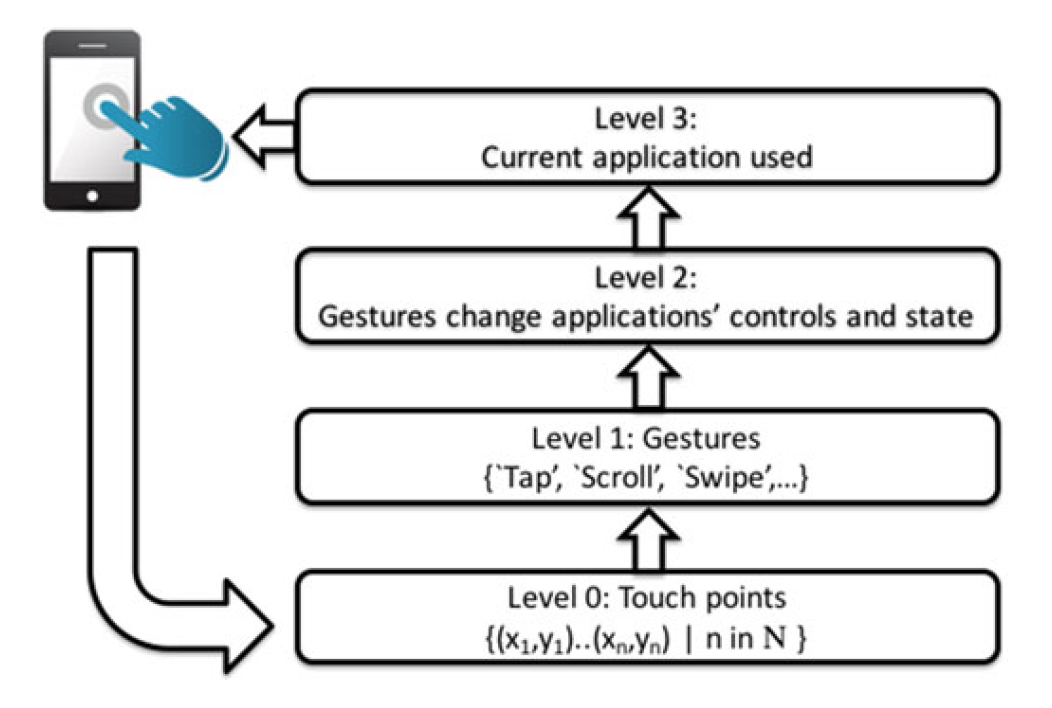
\includegraphics[width=0.7\textwidth]{fig-hsi-level}
  \caption{Human-smartphone interaction levels (\cite{21_ciman_2})}
  \label{fig:hsi-level}
\end{figure}

While these two research papers provided valuable insight into a completely non-intrusive way of gathering user data for stress prediction which does not rely on any external devices other than smartphones, implementing its theory in reality is rather challenging. On the one hand, few mobile operating systems provide developers the freedom of tracking every gesture and keyboard input of the user. While on the other, gathering information on application usage greatly depends on the platform. It by no means rules out the possibility of building an application that is able to acquire such data, but it is likely to be an integrated one operating on both the OS level and application level. Therefore, it does not serve the goal of this thesis, where the chatbot is based on a light-weight open-source platform that has no access to users' phone data.

\section{Intrusiveness and Timing of Digital Intervention}\label{section:timing}
The timing of intervention is a choice that every designer of a chatbot has to make. Understandably, for a dialog system, the more frequently it interacts with the user, the more information it is likely to acquire, but the more intrusive it becomes, and vice versa. This section presents some of the previous research done in the area of timing.\bigskip

\noindent In a study on using reminders or prompts to improve user engagement, \citeauthor{25_timing_review} (\citeyear{25_timing_review}) made a systematic review on 14 studies with 9774 participants and came to the conclusion that technology-based strategies such as prompts can promote engagement, although most reviewed researches were conducted with relatively small sample size. It also pointed out that according to one study, notifications "sent to users shortly after they started using the digital intervention were more likely to engage users".\bigskip

\noindent While the previous study focused on better engaging users, \citeauthor{26_cost_interruption} (\citeyear{26_cost_interruption}) emphasized on the cost of interruptions that the interaction with mobile applications results in. The study was based on the Android operating system. The combination of a switch from one foreground application to another for some duration, and then a switchback is considered an interruption. A user study was conducted with the help of a dataset provided by an Android background service. It found out that the interruptions occur in a relatively small fraction of smartphone usage, but the impact per interruption is considerable, with delayed completion of tasks by up to 4 times. This finding enhances the assumption that the timing of digital intervention is crucial not only in keeping users attached to the application but also in interfering with less of the users' normal tasks.\bigskip

\noindent It is therefore obvious that system designers and software developers need to find ways to determine the best time to interact with the user, and one approach is getting to know the users' needs. In order to get the notification time right, \citeauthor{27_oguz} (\citeyear{27_oguz}) developed a system to predict the time when a user is likely to eat based on historical data of eating time. He collected data on a daily basis, and selected five features, i.e. day of the week, the number of meals the user has had on the day, the number of snacks, the type of the latest entry (meal or snack), and the time of that entry. The target to predict was the time until the next entry, i.e. when the user is most likely to eat next. Machine learning was used to train the regression models for prediction, where random forest and linear regression had proven to be the most prominent models. Both qualitative and quantitative measures showed that the models brought with high accuracy in predicting when a user would want to eat.

\section{Review of a Similar System}
With all the insight into the intrusiveness and timing of intervention, this section presents a very brief review of a system (\cite{31_marija}) which is similar, both in terms of purposes and in terms of scope, with the chatbot that I developed.

\citeauthor{31_marija} proposed a method to estimate the likelihood of a user overeating under the influence of stress, and support the user with a dialog system. Like this thesis, \citeauthor{31_marija}'s result can also be potentially used to design recommender systems, or be used by therapists for making dietary plans. Instead of using a machine learning approach that is popular among similar dialog systems, the author has chosen the Eating and Appraisal Due to Emotions and Stress (EADES) Questionnaire (\cite{33_eades}) which helps to determine the likelihood of stress eating. In addition, physical data of the user such as gender, age, weight, and height were extracted. Combining the data, a lexical analysis determines the stress level of the user and what comes next in the conversation.

\citeauthor{31_marija}'s study provided useful insight into finding the relations between stress and eating using conversations and reacting to it. However, there are limitations in a number of areas. First, it only took overeating but not undereating into consideration. Second, the system was not tested among users, leaving the resulting model not evaluated. Last but not the least, the questionnaire contains 49 questions, which takes a considerable amount of time for a user to finish, which is, based on the theories presented earlier in this section, potentially intrusive to the user.\bigskip

\noindent This thesis addresses the limitations of the above study, providing a relatively non-intrusive chatbot that was tested with and evaluated by users.
